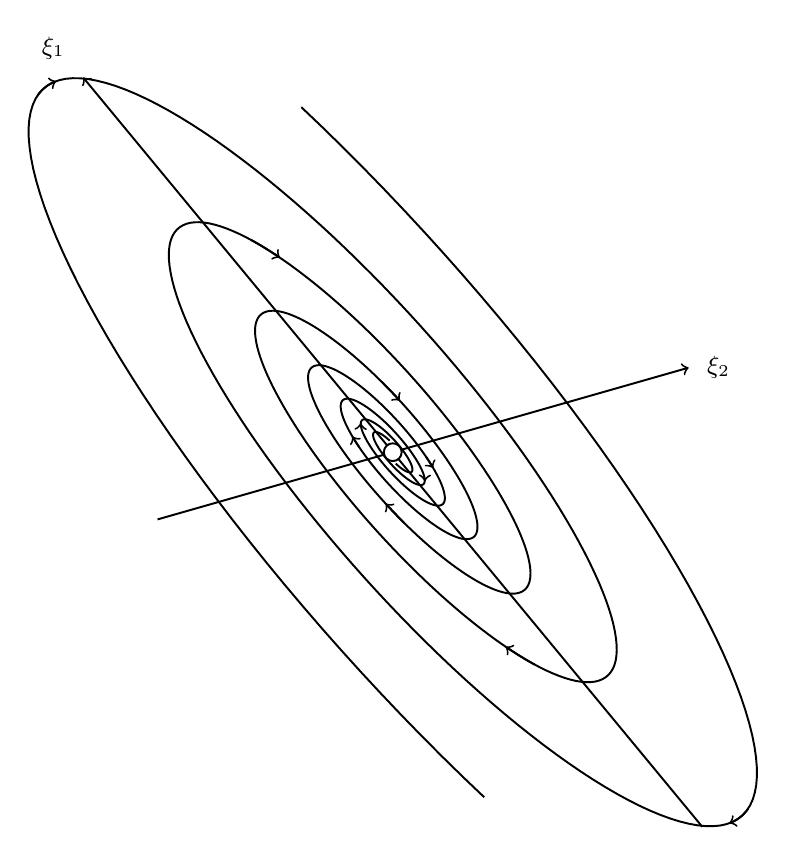
\begin{tikzpicture}[scale=2.1413,font=\small,x=0.9cm,y=0.9cm,line width=0.7pt]
  % Two centrally inverted stable logarithmic spirals under one affine map.
  % P=[(-0.95,1.15)^T,(0.42,0.12)^T], rho=3 exp(-0.0027(a-55)).
  \foreach \sgn in {-1,1} {
    \draw plot[domain=55:1315,samples=500,variable=\a]
      ({\sgn*3*exp(-0.0027*(\a-55))*(-0.95*cos(\a)+0.42*sin(\a))},
       {\sgn*3*exp(-0.0027*(\a-55))*(1.15*cos(\a)+0.12*sin(\a))});
    \foreach \j in {110,330,550,770,990} {
      \draw[->] plot[domain={55+\j-5}:{55+\j+5},samples=9,variable=\a]
        ({\sgn*3*exp(-0.0027*(\a-55))*(-0.95*cos(\a)+0.42*sin(\a))},
         {\sgn*3*exp(-0.0027*(\a-55))*(1.15*cos(\a)+0.12*sin(\a))});
    }
  }
  % Original coordinate images only: positive xi_1 is NW, positive xi_2 is NE.
  \draw[->] (2.04,-2.469)--(-2.04,2.469);
  \draw[->] (-1.55,-0.443)--(1.95,0.557);
  \fill[white] (0,0) circle (1.5pt);
  \draw (0,0) circle (1.5pt);
  \node[above left=3pt] at (-2.04,2.469) {$\xi_1$};
  \node[right=3pt] at (1.95,0.557) {$\xi_2$};
\end{tikzpicture}
